\chapter{Integration by Parts}

The product rule tells you how to differentiate a product of two functions. Run it backwards, and you get one
of the most useful tricks in all of integration. In the Methods of Integration chapter, you integrated rational
functions and powers of trigonometric functions. This chapter handles products like $x e^x$ and $x \sin x$,
and uses them to find the mean of a continuous probability distribution.

\section{Integration by Parts}

Recall the Product Rule for derivatives:

$$\frac{d}{dx} \left[ f(x) \cdot g(x) \right] = f(x) \cdot g'(x) + f'(x) \cdot g(x)$$

If we integrate both sides, we find that:

$$f(x) \cdot g(x) = \int \left[ f(x) \cdot g'(x) + f'(x) \cdot g(x) \right]\,dx$$
$$f(x) \cdot g(x) = \int f(x)g'(x)\,dx + \int f'(x)g(x)\,dx$$

Rearranging, 

$$\int f(x)g'(x)\,dx = f(x)g(x) - \int f'(x)g(x)\,dx$$

This identity allows us to perform \textbf{integration by parts}
\index{integration by parts}, a powerful method that allows us to evaluate 
integrals of complex functions. 

\textbf{Example}: Evaluate $\int x \cos{x} \,dx$.

\textbf{Solution}: We may be tempted to try $u$-substitution, but that will not 
work because $\frac{d}{dx} \cos{x}$ is not proportional to $x$ and $\frac{d}{dx} 
x$ is not proportional to $\cos{x}$. Let us define $f(x) = x$ and $g'(x) = 
\cos{x}$. This implies $f'(x) = 1$ and $g(x) = \sin{x}$. Then we can say that:

$$\int x \cos{x} \,dx = \int f(x)g'(x)\,dx$$

Using the identity $\int f(x)g'(x)\,dx = f(x)g(x) - \int f'(x)g(x)\,dx$ and 
substituting for $f(x)$, $f'(x)$, $g(x)$, and $g'(x)$, we see that:

$$\int x \cos{x} \,dx = \left[ x \sin{x} \right] - \int 1 \cdot \sin{x}\,dx$$
$$= x \sin{x} - \int \sin{x}\,dx$$
$$= x \sin{x} - \left( -\cos{x}  + C \right) = x \sin{x} + \cos{x} + C$$

(recall that C is the integration constant). You can check your results by 
taking the derivative: you should get the original integrand back. Let us check 
our result in this case:
$$\frac{d}{dx} \left[ x \sin{x} + \cos{x} + C \right] = \frac{d}{dx} \left[x 
\sin{x} \right] + \frac{d}{dx} \cos{x}$$
$$= x \frac{d}{dx} \left( \sin{x} \right) + \sin{x} \frac{d}{dx} (x) - \sin{x}$$
$$= x \cos{x} +\sin{x} - \sin{x} = x \cos{x}$$

How did we choose that $f(x)$ should be $x$ and $g(x)$ should be $\sin{x}$ in 
the example above? In general, you want to choose such that the resulting 
integral is simpler than the one we started with. This means you want to choose 
$f$ such that $f'$ is \textit{less complex} or a \textit{lower order} than $f$. 

To illustrate this, let us re-evaluate the example above, but this time let $f(x) 
= \cos{x}$ and $g'(x) = x$. Then we can say that $f'(x) = -\sin{x}$ and $g(x) 
= \frac{1}{2}x^2$. Substituting this into the integration by parts identity, 
we find that:
$$\int x \cos{x} \,dx = \frac{1}{2}x^2 \cos{x} - \int -\frac{1}{2}x^2 \sin{x}\,dx$$

Now the integral on the right side is more complex than the one we started 
with (on the left)! A good general rule for integration by parts is that 
\textit{if} the two functions in the original integral are a polynomial and a 
sine or cosine function, set the polynomial to be $f(x)$ and the trigonometric 
function to be $g'(x)$. The polynomial will be differentiated and become 
\textit{less} complex, while integrating the trigonometric function will not make 
it \textit{more} complex. 

Integration by parts is valid for definite integrals as well. Mathematically, 
this means:

$$\int_a^b f(x)g'(x)\,dx = f(x)g(x)|_a^b - \int_a^b f'(x)g(x)\,dx$$

Which is the same as:

$$\int_a^b f(x)g'(x)\,dx = \left( f(b) g(b) \right) - \left( f(a) g(a) \right) 
- \int_a^b f'(x)g(x)\,dx$$

Let us see one more example that incorporates both $u$-substitution and 
integration by parts.

\textbf{Example}: Evaluate $\int \frac{\arcsin{\ln{x}}}{x}\,dx$

\textbf{Solution}: First, we notice that $\ln{x}$ and $\frac{1}{x}$ both 
appear in the integrand. Let us define $u = \ln{x}$. Then $du = \frac{dx}{x}$:

$$\int \arcsin{\ln{x}} \frac{dx}{x} = \int \arcsin{u}\,du$$

For integration by parts, if we let $\arcsin{u} = f(u)$ and $du = g'(u)$, it 
follows that $f'(u) = \frac{1}{\sqrt{1-u^2}}$ and $g(u) = u$. Then we can say 
that:
$$\int \arcsin{u}\,du = \arcsin{u} \cdot u - \int \frac{u}{\sqrt{1-u^2}}\,du$$

We can use $u$-substitution again to evaluate the second integral (we will use 
$v$, since we have already said that $u = \ln{x}$). Let $v = 1-u^2$, which 
means that $\frac{dv}{2} = (-u)du$. Substituting:

$$= u \cdot \arcsin{u} + \int \frac{1}{2\sqrt{v}}\,dv = u \cdot \arcsin{u} + 
\sqrt{v}$$

Substituting back for $v$:

$$= u \cdot \arcsin{u} + \sqrt{1-u^2}$$

And substituting back for $u$:

$$= \ln{x} \cdot \arcsin{\ln{x}} + \sqrt{1 - \ln^2{x}} + C$$

\begin{Exercise}[label=int_meth3]
Let $f$ be a function such that $\int f(x) \sin{x}\,dx = -f(x)\cos{x} 
+ \int 4x^3 \sin{x}\,dx$. Give a possible expression for $f(x)$. 
\end{Exercise}

\begin{Answer}[ref=int_meth3]
This question takes the form of integration by parts. That is, $\int 
f(x)g'(x)\,dx = f(x)g(x) - \int g(x)f'(x)\,dx$. If we let $g(x) = 
-\cos{x}$, then $g'(x) =\sin{x}$. The structure of the equation 
implies that $f'(x) = 4x^3$ and therefore that $f$ could be $f(x) = 
x^4$. 
\end{Answer}

\begin{Exercise}[label = int_meth5]
Evaluate the following integrals using integration by parts:
\begin{enumerate}
\item $\int_0^{1} x \sin{\frac{\pi}{2} x}\,dx$
\item $\int e^{\theta} \cos{\theta}\,d\theta$
\item $\int (1-t)^2 \cos{\beta t}\,dt$
\end{enumerate}
\end{Exercise}

\begin{Answer}[ref = int_meth5]
\begin{enumerate}
\item $\frac{4}{\pi^2}$. Let $f = x$ and $g' = \sin{\frac{\pi}{2}x}dx$. Then 
$f' = dx$ and $g = -\frac{2}{\pi}\cos{\frac{\pi}{2}x}$. Which implies that 
$\int_0^{1} x \sin{\frac{\pi}{2} x}\,dx = \left[ \frac{-2x}{\pi}\cos{\frac{\pi}{
2}x} \right]_{x=0}^{x=1} - \int_0^1 \frac{-2}{\pi}\cos{\frac{\pi}{2}x}\,dx$. 
Evaluating $\left[ \frac{-2x}{\pi}\cos{\frac{\pi}{2}x} \right]_{x=0}^{x=1} = 
\left( \frac{-2}{\pi}\cos{\frac{\pi}{2}} \right) - \left(0 \cos{0} \right) = 0 
- 0 = 0$. Therefore, $\int_0^{1} x \sin{\frac{\pi}{2} x}\,dx = \int_0^1 \frac{2
}{\pi}\cos{\frac{\pi}{2}x}\,dx = \frac{2}{\pi} \left[\frac{2}{\pi}\sin{\frac{
\pi}{2}x} \right]_0^1 = \frac{4}{\pi^2} \left[ \sin{\frac{\pi}{2}} - \sin{0} 
\right] = \frac{4}{\pi^2}$. 
\item $\frac{e^{\theta}}{2} \left( \sin{\theta} + \cos{\theta} \right)$. Let 
$f = e^{\theta}$ and $g' = \cos{\theta} d\theta$. Then $f' = e^{\theta} 
d\theta$ and $g = \sin{\theta}$ and according to integration by parts $\int 
e^{\theta} \cos{\theta}\,d\theta = e^{\theta} \sin{\theta} - \int e^{\theta} 
\sin{\theta}\,d\theta$. We can also evaluate $\int e^{\theta} \sin{\theta}\,
d\theta$ using integration by parts. Let $f = e^{\theta}$ and $g' = \sin{
\theta} d\theta$. Then $f' = e^{\theta} d\theta$ and $g = -\cos{\theta}$ and 
according to integration by parts $\int e^{\theta} \cos{\theta}\,d\theta = e^{
\theta} \sin{\theta} - \left[ -e^{\theta} \cos{\theta} - \int -e^{\theta} \cos{
\theta}\,d\theta \right] = e^{\theta} \sin{\theta} + e^{\theta} \cos{\theta} - 
\int e^{\theta} \cos{\theta}\,d\theta$. We can rearrange this to solve for 
$\int e^{\theta} \cos{\theta}\,d\theta$: $2\int e^{\theta} \cos{\theta}\,
d\theta = e^{\theta} \sin{\theta} + e^{\theta} \cos{\theta} \rightarrow \int 
e^{\theta} \cos{\theta}\,d\theta = \frac{e^{\theta}}{2} \left(\sin{\theta} + 
\cos{\theta} \right)$. 
\item $\frac{(1 - t)^2}{\beta} \sin{\beta t} + \frac{2(t - 1)}{\beta ^2} \cos{
\beta t} - \frac{2}{\beta ^3} \sin{\beta t}$. Let $f = (1 - t)^2$ and $g' = 
\cos{\beta t}dt$. Then $f' = -2(1-t)dt$ and $g = \frac{1}{\beta} \sin{\beta t
}$. Then using integration by parts $\int (1-t)^2 \cos{\beta t}\,dt = \frac{(1 
- t)^2}{\beta} \sin{\beta t} - \int \frac{(-2)(1-t)}{\beta} \sin{\beta t}\,dt 
= \frac{(1 - t)^2}{\beta} \sin{\beta t} + \frac{2}{\beta} \int (1 - t) \sin{
\beta t}\,dt$. We use integration by parts again to evaluate $\int (1 - t) 
\sin{\beta t}\,dt$. Let $f = 1 - t$ and $g' = \sin{\beta t}dt$. Then $f' = 
-dt$ and $g = -\frac{1}{\beta} \cos{\beta t}$. Then $\int (1 - t) \sin{\beta t}
\,dt = (1 - t) \left( -\frac{1}{\beta} \right) \cos{\beta t} - \int \left( -
\frac{1}{\beta} \right) \cos{\beta t}\,-dt = \frac{t - 1}{\beta} \cos{\beta t} 
- \int \frac{\cos{\beta t}}{\beta}\,dt = \frac{t - 1}{\beta} \cos{\beta t} - 
\frac{1}{\beta ^2} \sin{\beta t}$. Substituting this back in for $\int (1 - t)
\sin{\beta t}\,dt$, we see that $\int (1 - t)^2 \cos{\beta t}\,dt = \frac{(1-t)
^2}{\beta} \sin{\beta t} + \frac{2}{\beta} \left[ \frac{t - 1}{\beta} \cos{
\beta t} - \frac{1}{\beta ^2} \sin{\beta t} \right] = \frac{(1 - t)^2}{\beta} 
\sin{\beta t} + \frac{2(t - 1)}{\beta ^2} \cos{\beta t} - \frac{2}{\beta ^3} 
\sin{\beta t}$.
\end{enumerate}
\end{Answer}

\section{Application: The Mean of a Probability Distribution}\index{expected value!continuous}
Integration by parts has an important use in probability. How can we find the average (mean) of a variable with a given probability 
distribution function? Consider the example of transaction processing times. 
If we knew the total time spent processing transactions and the total number 
of customers, then the mean processing time would be the total processing time 
divided by the total number of customers. 

Suppose we have a PDF that describes processing time for electronic 
transactions, $f(t)$, where $t$ is processing time and $f(t)$ is the 
probability that an individual transaction takes a particular amount of time, 
$t$. Electronic transactions are fast, and we can assume no transaction takes longer than 250 milliseconds, so we restrict the domain of $f(t)$ to $0 \leq t \leq 250$. We can divide the PDF into intervals of width $\Delta t$ (see figure 
\ref{fig:mean}). 

\begin{figure}[H]
    \centering
    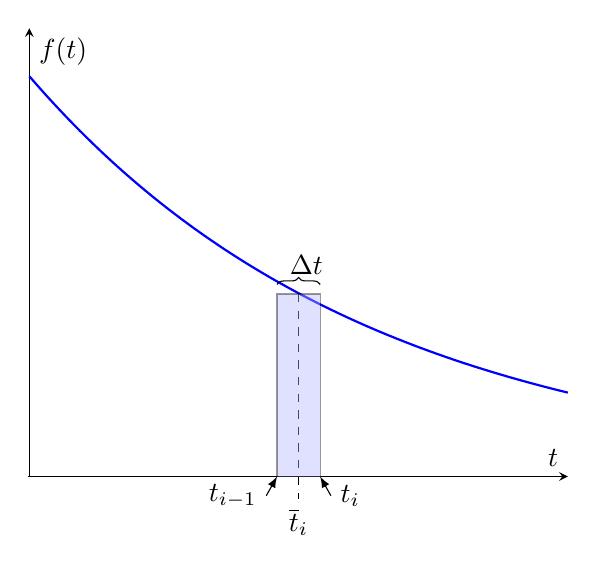
\begin{tikzpicture}
	\begin{axis}[xmin = -0.5, xmax = 250, ymin = 0, ymax = 0.007, axis lines = 
	center, xlabel = $t$, ylabel = $f(t)$, ticks = none, clip = false]
		\addplot[blue, thick, domain = 0:250, samples = 300] {(1/160)*e^(-1*x/160)};
        \draw[black, dashed] (125, 0.00285) -- (125, -0.00035) node[below] {
        $\overline{t}_i$};
        \draw[black, fill = blue!30, opacity = 0.4] (115, 0) rectangle 
        (135, 0.00285);
        \draw[latex-] (115, 0) -- (110, -0.0003) node[left] {$t_{i-1}$};
        \draw[latex-] (135, 0) -- (140, -0.0003) node[right] {$t_i$};
        \draw[decorate, decoration = brace] (115, 0.003) -- (135, 0.003) 
        node[above, xshift = -5] {$\Delta t$};
		\end{axis}
	\end{tikzpicture}
    \label{fig:mean}
    \caption{The probability that an individual transaction takes between 
    $t_{i-1}$ and $t_i$ seconds is approximated by the shaded area}
\end{figure}

If a total of $N$ transactions are processed, then the number of transactions 
that take between $t_{i-1}$ and $t_i$ is the probability of a transaction 
taking between $t_{i-1}$ and $t_i$ times $N$. That probability is approximately $f(\overline{t}_i) \Delta t$, and so the number of transactions taking between 
$t_{i-1}$ and $t_i$ is $Nf(\overline{t}_i) \Delta t$. Each of these 
transactions took approximately $\overline{t}_i$, and therefore the total 
processing time for these transactions is the number of transactions multiplied
by the processing time:
$$\overline{t}_i \left[ N f(\overline{t}_i) \Delta t \right]$$

To find the total processing time for all transactions, we would add up the 
total processing time for each interval:
$$\sum_{i = 1}^n N \overline{t}_i f(\overline{t}_i) \Delta t$$

And to find the average or mean processing time, we would divide this sum by 
the total number of customers, $N$:
$$\text{mean processing time} = \sum_{i = 1}^n \overline{t}_i f(\overline{
t}_i) \Delta t$$

Taking the limit as $n \to \infty$, the sum becomes an integral:
$$\text{mean processing time} = \int_0^{250} t \cdot f(t)\,dt$$

Recall that we use $\mu$ to represent the mean. Therefore, for a general PDF, 
$f(x)$, the mean is given by:
$$\mu = \int_{-\infty}^{\infty} x \cdot f(x)\,dx$$

\textbf{Example}: Find the mean value of the general exponential PDF, 
$$f(x) = 
\begin{cases}
0,&\text{if }x < 0\\
ce^{-cx},&\text{if }x \geq 0
\end{cases}$$

\textbf{Solution}: Applying the definition of the mean:
$$\mu = \int_{-\infty}^{\infty} xf(x)\,dx = \int_0^{\infty} xce^{-cx}\,dx$$
$$= -xe^{-cx}|_{x = 0}^{x = \infty} - \int_0^{\infty} -e^{-cx}\,dx$$
$$= 0 + \left[-\frac{1}{c}e^{-cx} \right]_{x = 0}^{x = \infty} = \frac{1}{c}$$

And since $\mu = 1/c$, we can re-write the general exponential PDF in terms of 
the mean:
$$f(x) = 
\begin{cases}
0,&\text{if }x < 0\\
\mu^{-1}e^{-x/\mu},&\text{if }x \geq 0
\end{cases}$$

\begin{Exercise}[title = {Onset of Symptoms}, label = symptoms]
Researchers find that the time between infection by the COVID virus and the 
onset of symptoms can be described by the PDF:
$$f(t) = 
\begin{cases}
\frac{1}{595} te^{-0.04t},&\text{if }0 \leq t \leq 120\\
0,&\text{otherwise}
\end{cases}$$

What is the mean time between infection and the onset of symptoms?
\end{Exercise}

\begin{Answer}[ref = symptoms]
$$\mu = \int_{-\infty}^{\infty} tf(t)\,dt = \frac{1}{595} \int_{0}^{120} t^2 e^{-0.04t}\,dt$$

Integrate by parts twice, or use the antiderivative
$$\int t^2 e^{-at}\,dt = -e^{-at}\left(\frac{t^2}{a} + \frac{2t}{a^2} + \frac{2}{a^3}\right)$$
with $a = 0.04$. Evaluating from $0$ to $120$ gives
$$\mu = \frac{1}{595}\left(31250 - 541250\,e^{-4.8}\right) = \frac{6250 - 108250\,e^{-4.8}}{119} \approx 45.04$$

Therefore, the mean time until the onset of symptoms is approximately 45 hours.
\end{Answer}
